\documentclass[12pt,preprint]{aastex}
\usepackage{amssymb,amsmath,mathrsfs,hyperref,datetime}

\newcommand{\datavector}[1]{\boldsymbol{#1}}
\newcommand{\data}{\datavector{y}}
\newcommand{\datum}{\data_i}
\newcommand{\truedatum}{\data_{{\rm true}, i}}
\newcommand{\noiselessdata}{\tilde{\data}}
\newcommand{\noiselessdatum}{\tilde{\datum}}
\newcommand{\xdcov}{\datavector{V}_j}
\newcommand{\datacov}{\datavector{C}}
\newcommand{\postcov}{\tilde{\datacov}_{i, j}}
\newcommand{\vmu}{\datavector{\mu}}
\newcommand{\postmu}{\tilde{\vmu}_{i, j}}
\newcommand{\datumcov}{\datacov_i}
\newcommand{\transpose}{{\rm T}}
\newcommand\ttt[1]{{\texttt{#1}}}
\newcommand\rf[1]{{\bf [RF: #1]}}

\def\urltilda{\kern -.15em\lower .7ex\hbox{\~{}}\kern .04em}

\pdfoutput=1

\begin{document}

\title{Joint photometric modeling for improved measurements in imaging
surveys.}
\author{Ross~Fadely\altaffilmark{1} \&
        David~W.~Hogg\altaffilmark{1,2}}
\altaffiltext{1}{Center~for~Cosmology~and~Particle~Physics,
Department~of~Physics, New~York~University, 4~Washington~Place, New~York,
NY 10003, USA}
\altaffiltext{2}{Max-Planck-Institut f\"ur Astronomie, K\"onigstuhl 17, 69117
Heidelberg, Germany}


%%%%%%%%%%%%%%%%%%%%%%%%%%%%%%%%%%%%%%%%%%%
%
% Abstract
%
%%%%%%%%%%%%%%%%%%%%%%%%%%%%%%%%%%%%%%%%%%%
\begin{abstract}
Large scale astronomical imaging surveys have fundamentally changed our 
understanding of the cosmos, and promise to continue to do so with forthcoming 
surveys like the Large Synoptic Survey Telescope which will provide greater 
volumes of data at increasingly fainter detection limits.  In order to extract
the most science out of such costly missions, it is important to continually
explore ways to improve the means by which photometric measurements are made.
Historically, photometric measurements are made on a per object basis under
our understanding of the characteristics of the telescope, instruments, and
astronomical sources.  We argue that it is possible to improve the quality of
such photometric measurements by building models which incorporate the shared
similarity of sources.  As a demonstration, we use Extreme Deconvolution (XD)
to model the joint distribution of photometric quantities measured by SDSS in
Stripe 82.  Using single epoch data, we show that our joint XD model makes
predictions that more closely resemble the coadded Stripe 82 data.  Looking
at the difference between the psf and model magnitudes in the single epoch and 
coadded data, the average error is XX at $r\sim21$ versus an average of XX
for our XD posteriors.  In the case of the CMDs of globular clusters, we show
that the XD posteriors lessen the presence of misclassified galaxies and
present a narrower stellar locus.  We suggest a number of improvements that
can be made to provide improved photometric inferences.
\end{abstract}

%%%%%%%%%%%%%%%%%%%%%%%%%%%%%%%%%%%%%%%%%%%
%
% Section - Introduction
%
%%%%%%%%%%%%%%%%%%%%%%%%%%%%%%%%%%%%%%%%%%%
\section{Introduction}

Large imaging surveys of parts (or the full) sky are one main modes in which
modern astronomers study the universe.  Whether conducted on the ground (e.g.,
SDSS, UKIDSS, NEWFIRM, VLA, etc.) or in space (GALEX, WISE, XMM?, etc.), the
volume of such surveys provides both strong statistical samples of objects and
also the potential for new discoveries.  For instance, the Sload Digital Sky
Survey (optical $ugriz$, $r\lesssim 22$) \citep{york00} was first dataset able
to describe the quasar luminosity function (CITE?) while also enabling the 
discovery of new streams and satellites around the Milky Way (CITE).


%%%%%%%%%%%%%%%%%%%%%%%%%%%%%%%%%%%%%%%%%%%
%
% Section - Method
%
%%%%%%%%%%%%%%%%%%%%%%%%%%%%%%%%%%%%%%%%%%%
\section{Extreme Deconvolution}

Our goal is to construct a model of the joint distribution of the space of
possible photometric measurements.  The key idea is that once we have learned
what the underlying distribution can be, we can utilize this knowledge as a
prior distribution over what the set of \emph{true} observations should be for
a given object.  That is, for each datum we want to construct the posterior
for the true photometric quantities -

\begin{eqnarray}\displaystyle
p(\truedatum | \datum) & \propto & p(\datum | \truedatum) p(\truedatum) \\
                                         & \propto & \frac{1}{\sqrt{2\pi\det{|\datumcov|}}} \exp \left (-\frac{1}{2}(\datum - \truedatum)^\transpose \datumcov^{-1}(\datum - \truedatum) \right ) p(\truedatum)
\quad ,
\label{eqn:posterior}
\end{eqnarray}

\noindent where $\datum$ is the observed vector of photometric measurements, 
$\truedatum$ is the set of values we would have observed in the absense of
noise, and $\datumcov$ is the covariance for the observation which is
constructed from our (e.g, the survey's) noise estimates.  The distribution 
$p(\truedatum)$ is the prior distribution we wish to learn, and the likelihood
$p(\datum | \truedatum)$ is assumed to be Gaussian.  Since we are learning the
prior distribution from a set of many observations, this is refered to as a
multilevel or hierarchical model.

The art in building a hierachical model is deciding the structure of the
distributions involved -- how distributions are parameterized, what is held
fixed or considered know, and what the relationships are between the various
distributions.  We believe the distribution of $p(\truedatum)$ can be quite 
complex, and it is not obvious what the right description of the distribution
might be.  For these reasons, we choose to use Extreme Deconvolution (XD)
\citep{bovy09}.  XD is a simple but powerful and flexible model which models
the density of the data as a Mixture of Gaussians, accounting for the 
measurement errors of the observations.  In short, XD learns a model for which 
each datum is drawn from an underlying distribution which is convolved by the 
specified noise estimates.

After inference, the XD mixture provides an estimation for the `noiseless' (or
less noisy) distribution of the data:

\begin{eqnarray}\displaystyle
p(\noiselessdata) = \sum_j^K \frac{\alpha_j}{\sqrt{2\pi\det{|\xdcov|}}} \exp \left (-\frac{1}{2}(\noiselessdata - \vmu_j)^\transpose \xdcov^{-1}(\noiselessdata - \vmu_j) \right )
\quad .
\label{eqn:noiseless}
\end{eqnarray}

\noindent From here, we assume that the prior for $\truedatum$ is
$p(\noiselessdata)$.  Doing so, we consider the analysis here akin to an 
`empirical' heirarchical model -- the prior is not learned simultaneously with
the posterior but rather is learned separately from the collection of
observations.

Since $p(\noiselessdata)$ is a sum of Gaussian densities, and we multiply this
by a Gaussian likelihood, the posterior is also a sum of Gaussians.  That is,
the posterior for the true value of the observation is

\begin{eqnarray}\displaystyle
p(\truedatum | \datum) & \propto & \sum_j^K \frac{\alpha_j}{\sqrt{2\pi\det{|\postcov|}}} \exp \left (-\frac{1}{2}(\truedatum - \postmu)^\transpose \postcov^{-1}(\truedatum - \postmu) \right ) \\
{\rm where,}\\
\postcov & = & (\datumcov^{-1} + \xdcov^{-1})^{-1} \quad {\rm and,} \\
\postmu & = &  \postcov^{-1} (\datumcov^{-1} \datum + \xdcov^{-1} \vmu_j)
\label{eqn:posterior}
\end{eqnarray}

\section{Data and Model Considerations}

To demonstrate the utility of our approach, we focus on the $ugriz$
photometric data provided by SDSS' Data Release 10 \citep[DR10,][]{?} and
Stripe 82 \citep[S82,][]{annis14, others?}.  Here, our primary goal is to
provide better estimate of the dereddened PSF and model magnitudes observed by
SDSS.  More specifically, we aim to model the distribution of the $r$ band PSF
magnitudes, the $u-g$, $g-r$, $r-i$, and $i-z$ model colors, and the different
between PSF and model magnitudes in the $ugriz$ bands.  Thus, are fiducial 
models aim to understand the distribution of 10 measurements or `features' per 
observed source.

In DR10, we randomly select 30k `stars' and `galaxies' (\ttt{type} $= 6, 3$)
which PSF $r$ magnitudes between 18 and 22, which are \ttt{Primary}
photometric observations, and which have clean
photometry\footnote{Observations which are not true in \ttt{EDGE},
\ttt{NOPROFILE}, \ttt{PEAKCENTER}, \ttt{NOTCHECKED}, \ttt{PSF\_FLUX\_INTERP},
\ttt{SATURATED}, \ttt{BAD\_COUNTS\_ERROR}, \ttt{DEBLEND\_NOPEAK},
\ttt{INTERP\_CENTER}, or \ttt{COSMIC\_RAY}, and is detected in
\ttt{BINNNED1}.}.  The even number of stars and galaxies selected for our
sample is to mitigate any biases we might induce by favoring one population
over the other.  For purpose of comparing lower signal-to-noise obversations
to ones of higher quality, we also select a similar set of observations from
the S82 coadd \citep{annis14}.  S82 is unique in the SDSS dataset as it is one
of the few region of the sky for which on average $\sim 20$ epochs of imaging
have been taken.  As a result, the median $r$ PSF magnitude uncertainty in a
single epoch is BLAH compared to a median of BLAH for the coadded data (c.f, 
\ref{fig:error_rates}).  For the results presented below, we have trained our
XD model on the DR10 data described above and use this model to calculate
posteriors for both DR10 and S82 single epoch data.

For our XD model, we must specify the number of components in the XD mixture.
Since our goal is simply to demonstrate the utility of our method, we set the 
number somewhat arbitrarily to 32.  We also tweak the XD algorithm presented in
\citet{bovy09} by allowing the user to specify the mean value of a feature,
as well as inforce that the covariance for a feature to be axis aligned
(diagonal elements only).  For PSF minus model magnitude features, we force
the mean to be zero and for the covariance to be axis aligned since this is
expected for unresolved sources. Since there are also extended sources in the
data, we only do so for $N_{\rm point}$ components of the mixture.  Again,
somewhat arbitrarily we set this number to 16.  We have set the number of
components in the mixture (both in total and for unresolved sources) to
sensible numbers given the amount of data used, and seem to have adequate
performance for our purposes.  If this was done in a science quality or
survey data product setting, we recommend setting these parameters via cross
validation with data at higher signal to noise.  Finally we note that we 
apply a small amount of regularization to the covariance of the mixture
components, exactly the same in nature to that of \citet{bovy10}.  In short, 
a small value $w$ is added to the diagonal of the covariances to prevent
singular matrices during the learning process.  We set $w$ to be 1\% of the 
smallest uncertainty measured in each feature, and find that this does not
significantly affect our final results.

\section{Results and Discussion}

We find the XD model provides a good understanding of the distribution of the 
data, and that the posteriors we compute are sensible, less noisy estimates of 
the observations.  To start, we examine the distribution of the XD mixture 
relative to the DR10 data.  In figure \ref{fig:contours} we show the contours 
of the $N_{\rm point}$ components along with data labeled as `star' in DR10,
and likewise for extended sources.  While its difficult to assess the quality
of the XD model from the plots, there are a few supporting points.  For the 
unresolved sources, the mixture prefers low variance in the value of $r$ PSF
minus model magnitudes which is in agreement we our intuition that stars
ought to be clustered around values of zero.  Second, the stellar locus in
color is clear and well tracked by the XD $N_{\rm point}$ components.  Though 
galaxies have less defining characteristics, it is clear that the XD mixture 
also tracks their distribution well.

\begin{figure}
\centering
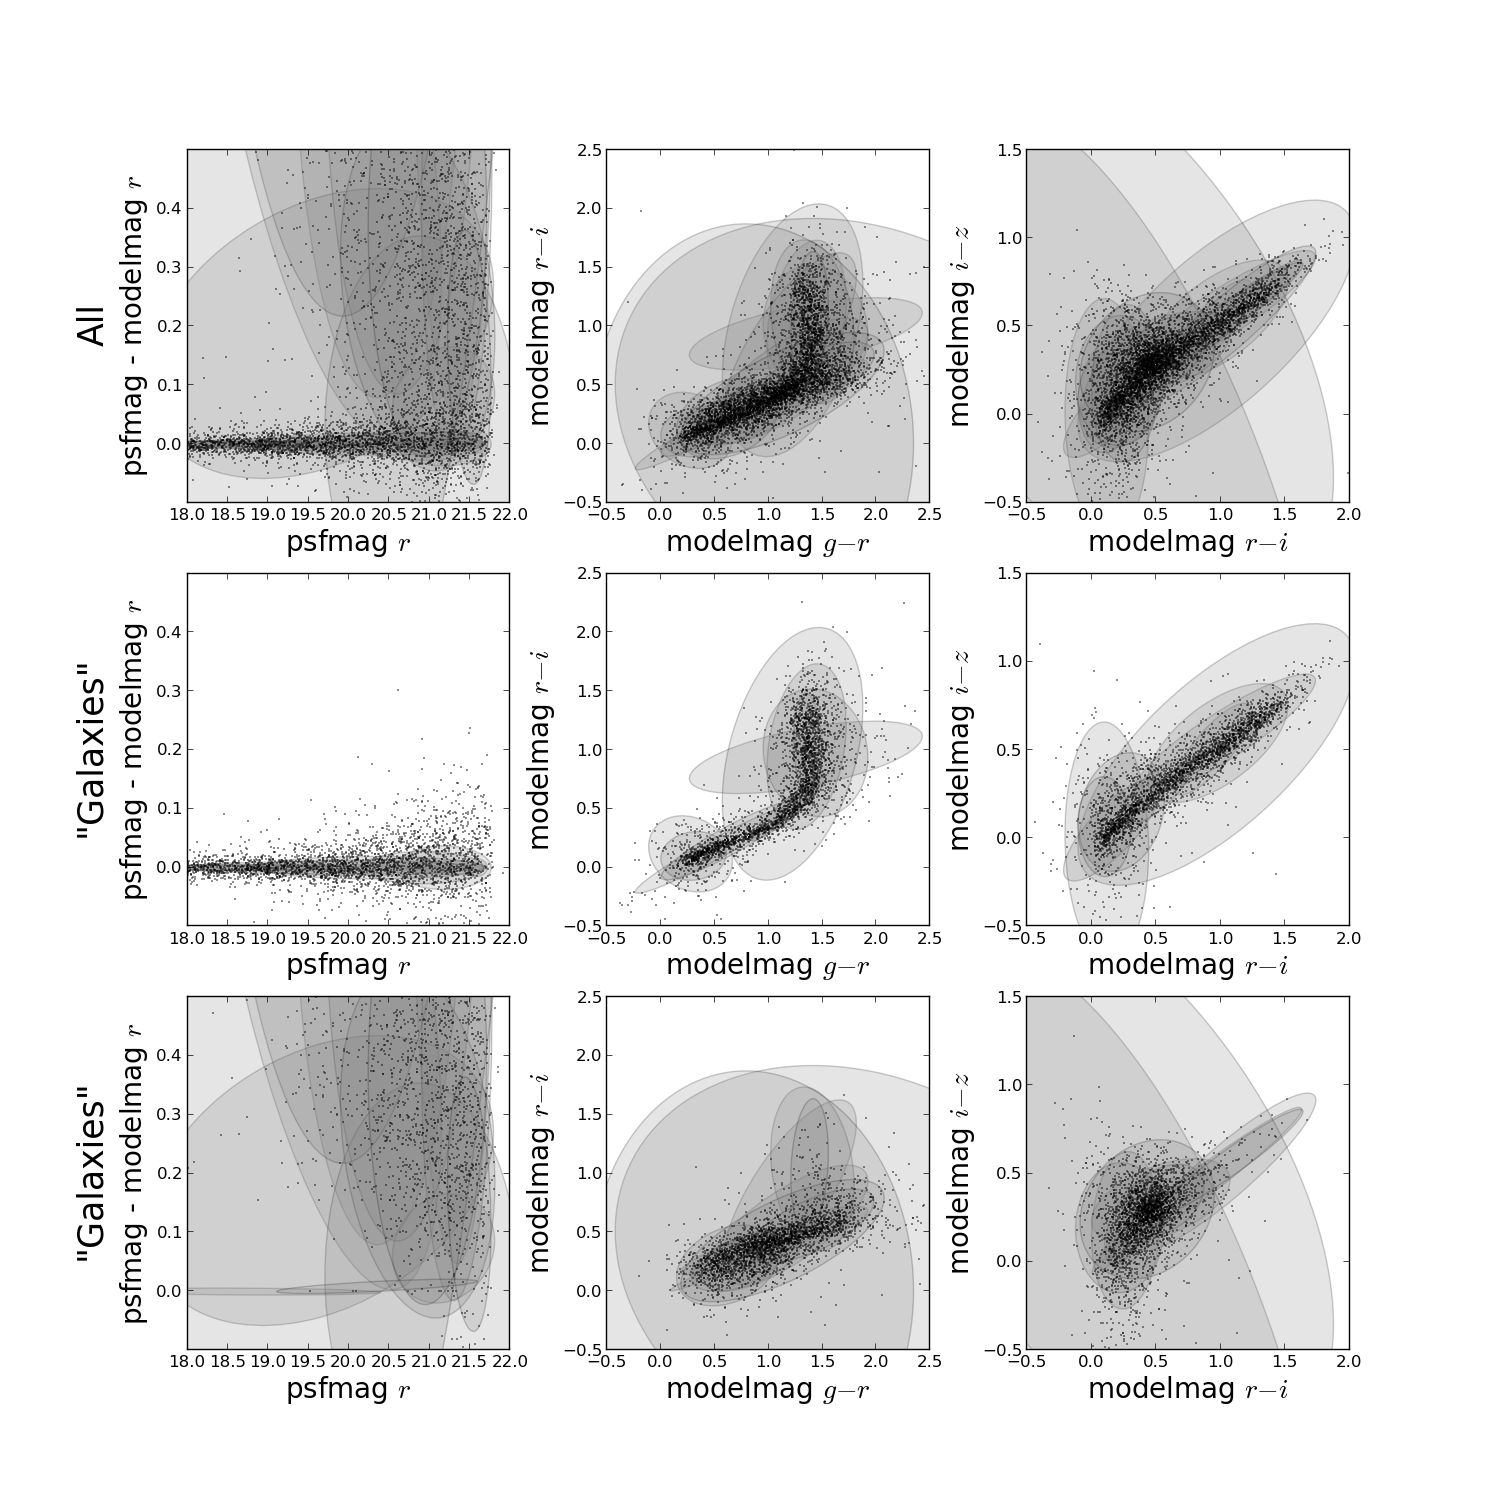
\includegraphics[clip=true, trim=1.5cm 0.5cm 1.5cm 0.5cm,
  width=16cm]{fig1.png}
\caption{Shown are three different projections of one tenth of the DR10
photometric data used (black points), with the top/bottom row corresponding
objects classified as stars/galaxies (\ttt{type} $=6, 3$).  Gray contours
indicate the different XD components.  For the top we only plot the
$N_{\rm point}$ components while in the bottom we plot the rest.  Note,
however, when we compute our model we do not use SDSS classifications -- all
data is modeled with the combination of both top and bottom contours.  Note
the components modeling psfmag minus modelmag for starlike objects prefer
small variance, and generally the model follows the data well.
}
\label{fig:contours}
\end{figure}

In figure \ref{fig:posteriors}, we show the posterior distributions for 3
stars and 3 galaxies at different magnitudes.

So far we have shown operationally that the XD model does sensible modeling of
the photometry and is more \emph{precise}, but it is important to ask whether
the posteriors are at all \emph{accurate}.  To do so, we rely on comparsions of
the posteriors we get for S82 single epoch data versus the data from the
coadd.  In figure \ref{fig:xx_plots}, we plot the different between the single
epoch and coadd data, as well as our XD posteriors versus the coadd.  We find
that the median of the residuals for our XD posteriors is consistent with
zero, indicating the model is not only precise but also accurate.  We note
this is true for all of the features we model.  Also obvious is the clear
improvement in the photometry over the single epoch data.

In SDSS, star-galaxy classification is accomplished by selecting objects a
small range of PSF minus model magnitudes and calling them stars.  In DR10,
the range is approximately\footnote{The actual algorith involves a combination
of this criterion for $gri$ bands.} $|r_{PSF} - r_{model}| < 0.145$ while the
S82 coadd criterion is $|r_{PSF} - r_{model}| < 0.03$.  In figure \ref{fig:pmm}
we show a normalized histogram of $r$ PSF minus model magnitudes around
$r=21$, for objects that are called stars in the coadd.  Note that our XD
posteriors dramatically tighten the distribution of objects around near zero,
and also indicate the present of interloping galaxies.

\end{document}
